%!TEX root = Tesi.tex

\section{RedBear Nano2}
Il dispositivo usato per implementare la funzione di sniffer è il Nano2 della società RedBear. Non più grande di una moneta (10mm x 18mm), ha un costo che si aggira attorno ai 30\$ .

\begin{figure}[H]
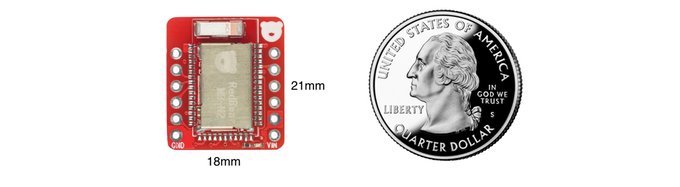
\includegraphics[width=300pt]{nano2_money}
\centering
\caption{RedBear Nano2, comparato con una moneta da 1/4 di dollaro.}
\end{figure}

Il nome in codice del modello è \lq MB-N2\rq ed integra al suo interno il chip della Nordic nRF52832, un'antenna integrata ed un totale di 32 pin di I/O\footnote{Input, Output: utilizzabili a piacimento come periferiche di ingresso o uscita} che offrono i servizi di UART, SPI, ADC e PWM.

\begin{figure}[H]
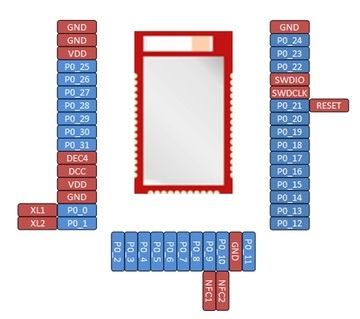
\includegraphics[width=250pt]{nano2_io}
\centering
\caption{Modulo SoC Nordic nRF52832 integrato nel RedBear Nano2.}
\end{figure}

\begin{samepage}
Il chip della Nordic Semiconductor nRF52832 Soc ha le seguenti caratteristiche
\begin{itemize}
\item[-] Processore ARM Cortex-M4F a 32 bit e 64 MHz.
\item[-] Bluetooth 4.2 certificato e compatibile con le specifiche 5.0 .
\item[-] NFC.
\item[-] 64 KB di ram.
\item[-] 512 KB di memoria Flash.
\item[-] FPU, unità di calcolo in virgola mobile.
\item[-] DSP, processore di segnale digitale.
\end{itemize}
\end{samepage}

Non disponendo di un'interfaccia standard per la comunicazione con un PC, il Nano2 necessita di una board di supporto sia per essere programmato, sia per comunicare informazioni a quest'ultimo.
La board che viene fornita assieme al Nano2 è chiamata DAPLink e disponibile nella versione 1.5 . Essa monta un processore ARM Cortex-M3 MCU ed è utilizzata oltre che per la programmazione, anche per il debug dei progetti su Nano2

\begin{figure}[H]
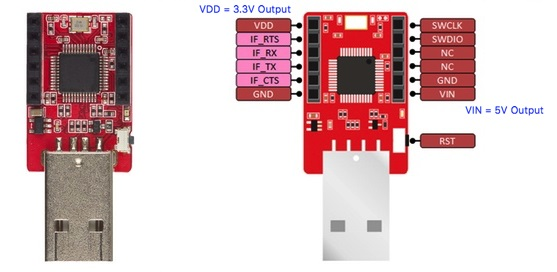
\includegraphics[width=330pt]{daplink}
\centering
\caption{Board DAPLink, un progetto open source del team ARM mbed.}
\end{figure}


